\documentclass[10pt,xcolor=dvipsnames]{beamer}
%\documentclass[10pt,xcolor=dvipsnames,handout]{beamer}
%\documentclass[10pt,xcolor=dvipsnames,handout]{beamer}
%\usepackage{pstricks}
%\usetheme{Boadilla}
%\usepackage{babel}
%\makeatother

%%%%%%%%%%%%%%%%%%%%%%%%%%%%%%%%%%%%%%%%%%%%%%%%%%%%%%%%%%%%%%%%%%%%%%%%%%%%%%%%%%%%%%%%%%%%%%%%%%%%%%%%%%%%%%%%%%%%%%%%
%PREAMBLE
%\useoutertheme{shadow}                 %at shadow at the top of the slide
\geometry{left=0.80cm,right=0.8cm}      %set margins
%\beamertemplatefootpagenumber          %add numbering of slides at the bottom
\usepackage{graphicx}                   %to import figures and graphics
\usepackage{booktabs}                   %to format tables nicely
\usepackage{hyperref}                   %to add hyperlink connections between slides
%\usepackage[overlay, absolute]{textpos} %to customize position of the slide content
\usepackage{epsfig}                    %to import .eps graphics
\usepackage{color}                      %to color text
\usepackage{amsmath,amssymb}            %fonts for symbolic math
%\usepackage{lmodern}                   %set font typesetting to lmodern
%\usepackage{times}                     %set font typesetting to times
\usepackage[latin1]{inputenc}           %set font typesetting
\usepackage{psfrag}
\usepackage{cancel}
\usepackage{cancel}
\usepackage{mathtools}
\usepackage{caption}
\usepackage{eurosym}
\usepackage{tikz}
\usetikzlibrary{trees}
\usepackage[outdir=./]{epstopdf}
\newcommand\tikzmark[1]{\tikz[remember picture,overlay]\coordinate (#1);}

\definecolor{cmu}{rgb}{0.76,0,0}
\renewcommand{\CancelColor}{\color{cmu}}

\renewcommand{\sfdefault}{cmss}         %switch font to serif cmss
%\usefonttheme[onlymath]{serif}          %still keep standard font for math whatever the changes
\usefonttheme{serif}
\def\widehrulefill{\leaders\hrule height 0.35pt\hfill} %define a line fill
\def\drawhline{\hrule height 0.6pt width 333pt}     %define a line
\def\no{\noindent}                      %define shortcut for no indent
\def\bul{\color{black}{$\bullet$}}      %define shortcut for full bullet item
\def\cir{\color{black}{$\circ$}}        %define shortcut for empty bullet item
\def\br{\color{black}{-}}               %define shortcut for a bar
\def\wbul{\color{white}{$\bullet$}}     %define shortcut for white full bullet item
\def\wcir{\color{white}{$\circ$}}       %define shortcut for white empty bullet item
\def\wx{\color{white}{x}}               %define shortcut for x bullet item
\def\bx{\color{black}{x}}               %define shortcut for x bullet item
\def\rx{\color{red}{x}}                 %define shortcut for x bullet item
\def\nor{\normalsize}                   %shorthand for normalsize
\def\bsk{\bigskip}                      %shorthand for skips
\def\msk{\medskip}
\def\ssk{\smallskip}
%\setbeamercovered{dynamic}             %transparent bullets in uncovering
\setbeamertemplate{frametitle}
{                                       %set the template for frame title
\bigskip
%\begin{center}
\definecolor{ltblack}{gray}{0.1}
\color{ltblack}{\large\textbf{{\insertframetitle} }}
%\large{\insertframetitle}
%\end{center}
}
%\definecolor{blue}{rgb}{0.7,0.1,0.7}                        %redefine blue color
%\definecolor{blue}{cmyk}{0,1,1,.3}
\definecolor{defblue}{rgb}{.2,.2,.7}                          %Default blue from beamer
\definecolor{purple}{rgb}{0.9,0.0,0.0}                        %redefine blue color
\setbeamertemplate{navigation symbols}{}                    %turn off navigation bar at the bottom of the page
%\useoutertheme{infolines}

%\setbeamercolor{footline}{fg=blue!40!white}
%\setbeamercolor{footline}{black} 
\setbeamertemplate{footline}{
% taken from theme infolines and adapted
%  \leavevmode%
  \hbox{%
  \begin{beamercolorbox}[wd=.49999\paperwidth,ht=2.25ex,dp=1ex,center]{}%
    \insertshortauthor \quad
  \end{beamercolorbox}%
  \begin{beamercolorbox}[wd=.49999\paperwidth,ht=2.25ex,dp=1ex,left]{}%
    \quad
    \insertshorttitle
    \hfill \quad\quad\quad\quad\quad
    \insertframenumber{} / \inserttotalframenumber
  \end{beamercolorbox}}

%  \begin{beamercolorbox}[wd=.333333\paperwidth,ht=2.25ex,dp=1ex,right]{}%
%%  \insertshortdate
%%        \hskip 10pt \insertframenumber{} / \inserttotalframenumber
%  \hspace*{2ex}
%  \end{beamercolorbox}}
  \vskip0pt
  }

\setbeamertemplate{itemize item}{\color{black} $\bullet$}   %redefine bullets for itemize level 1 (full bullet)
\setbeamertemplate{itemize subitem}{\color{black} $\circ$}  %redefine bullets for itemize level 2 (empty bullet)
\setbeamertemplate{itemize subsubitem}{\color{black} -}    %redefine bullets for itemize level 2 (empty bullet)
\setbeamerfont{itemize item}{size=\normalsize}
\setbeamerfont{itemize subitem}{size=\normalsize}
\setbeamerfont{itemize subsubitem}{size=\normalsize}

%\setbeamertemplate{section in toc}{\hspace*{1em}\color{black} $\bullet$ \inserttocsection \par}
%\setbeamertemplate{subsection in toc}{\hspace*{3em}\color{black} $\circ$ \inserttocsubsection \par}

\newcommand{\fs}{\mathcal{S}}
\newcommand{\RR}{\mathcal{R}}
\DeclareMathSymbol{\R}{\mathbin}{AMSb}{"52}


\newtheorem{defn}[theorem]{Definition}
\newtheorem{claim}[theorem]{Claim}
\newtheorem{assumption}[theorem]{Assumption}
\newtheorem{proposition}[theorem]{Proposition}

\usepackage[sc]{mathpazo}
%\usepackage{eulervm}

\setbeamertemplate{blocks}[rounded][shadow=false]
\makeatletter
\pgfdeclareverticalshading[lower.bg,upper.bg]{bmb@transition}{200cm}{color(0pt)=(lower.bg); color(4pt)=(lower.bg); color(4pt)=(upper.bg)}
\makeatother

\newenvironment<>{propblock}[1]{%
  \begin{actionenv}#2%
      \def\insertblocktitle{#1}%
      \par%
      \mode<presentation>{%
        \setbeamercolor{block title}{fg=white,bg=black}
       \setbeamercolor{block body}{fg=black,bg=black!5!white}
     }%
      \usebeamertemplate{block begin}}
    {\par\usebeamertemplate{block end}\end{actionenv}}


\setbeamercolor{unalert text}{fg=gray!50,bg=}
\setbeamercolor{normal text}{fg=black,bg=}
\setbeamercolor{alerted text}{fg=black,bg=}
\definecolor{cmu}{rgb}{0.76,0,0}
\setbeamercolor{button}{bg=black,fg=white}

\newcommand<>{\uncoverubrace}[2]{%
  \onslide#3 \underbrace{ \onslide<1->%
  #1%
  \onslide#3 }_{#2} \onslide<1->%
}
\newcommand<>{\uncoverobrace}[2]{%
  \onslide#3 \overbrace{ \onslide<1->%
  #1%
  \onslide#3 }^{#2} \onslide<1->%
}

\DeclareMathOperator*{\argmax}{arg\,max}

\title[Income Inequality]{\definecolor{ltblack}{gray}{0.1}\color{ltblack}\textbf{Breaking Down the Causes of Rising Income Inequality in the US}}
\author[Tengelsen ]{\texorpdfstring{\begin{columns}           
            \column{.3\linewidth}
            \centering
            Benjamin Tengelsen\\
            Hufflepuff
        \end{columns}
}{Tengelsen}
}
\date{Oct 26, 2016}


\begin{document}

\section*{Intro}
{
\setbeamertemplate{footline}{} 
\frame{\titlepage}
}
\addtocounter{framenumber}{-1}


% %%%%%%%%%%%%%%%%%%%%%%%%%%%%%%%%%%%%%%%%%%%%%%%%%%%%%%%%%%%%%%%%%%%%%%%%%%%%%%%%%%%%%%%%%%%%%%%%%%%%%%%%%%%%%%%%%%%%%%%%%%%%%%%%%%%%%
% \begin{frame}
% \frametitle{Some news \widehrulefill}
% \begin{itemize}
% \item Today is my birthday (29)
% \bsk
% \item I found out yesterday that I'm a Hufflepuff
% \bsk
% \item I found out yesterday that I'm a Hufflepuff
% \bsk
% \end{itemize}
% \end{frame}
% %%%%%%%%%%%%%%%%%%%%%%%%%%%%%%%%%%%%%%%%%%%%%%%%%%%%%%%%%%%%%%%%%%%%%%%%%%%%%%%%%%%%%%%%%%%%%%%%%%%%%%%%%%%%%%%%%%%%%%%%%%%%%%%%%%%%



%%%%%%%%%%%%%%%%%%%%%%%%%%%%%%%%%%%%%%%%%%%%%%%%%%%%%%%%%%%%%%%%%%%%%%%%%%%%%%%%%%%%%%%%%%%%%%%%%%%%%%%%%%%%%%%%%%%%%%%%%%%%%%%%%%%%
\begin{frame}
\frametitle{Question and Answer\widehrulefill}
\begin{itemize}
  \item What is driving the observed increase in income inequality?
  \begin{itemize}
    \smallskip
    \item Have the causes changed over time?
    \smallskip
    \item How much has each cause contributed? 
  \end{itemize}

  \bsk
  \item Empirical answers:
  \begin{itemize}
    \smallskip
    \item Technology: positive relationship (5 year lag)
    \smallskip
    \item Education: strong positive relationship (2 year lag)
    \smallskip
    \item Taxes: negative, but relatively weak relationship
    \smallskip
    \item Entrepreneurship: results vary drastically with lag length
  \end{itemize}

  \bsk
  \item Model: Not for today. 
\end{itemize}

\end{frame}
%%%%%%%%%%%%%%%%%%%%%%%%%%%%%%%%%%%%%%%%%%%%%%%%%%%%%%%%%%%%%%%%%%%%%%%%%%%%%%%%%%%%%%%%%%%%%%%%%%%%%%%%%%%%%%%%%%%%%%%%%%%%%%%%%%%



%%%%%%%%%%%%%%%%%%%%%%%%%%%%%%%%%%%%%%%%%%%%%%%%%%%%%%%%%%%%%%%%%%%%%%%%%%%%%%%%%%%%%%%%%%%%%%%%%%%%%%%%%%%%%%%%%%%%%%%%%%%%%%%%%%%%
\begin{frame}
\frametitle{Literature on Causes of Income Inequality \widehrulefill}
\begin{itemize}
  \smallskip
  \item 1990's - Is this skill-biased technological change (SBTC)? Human capital differences? Some combination?
  \begin{itemize}
    \smallskip
    \item Computers: Bound (AER,1992); David (QJE,1998); DiNardo and Card (JLE,2002); 
    \smallskip
    \item Human capital + SBTC: Acemoglu (QJE,1998); 
    \smallskip
    \item Demographics + Human capital: Heckman (RED,1998)    
  \end{itemize}

  \bsk
  \item Other theories: 
  \begin{itemize}
    \smallskip
    \item Taxes: Alvaredo et al (JEP,2013); Bakija et al (WP,2012)
    \smallskip
    \item Globalization: Krugman (Brookings,2008)
    \smallskip
    \item Finance boom/entrepreneurship: Bakija et al (WP,2012)    
    \smallskip
    \item Stigma:  Pickety and Saez (QJE,2003); Atkinson et al (JEL,2011)  
  \end{itemize}
\end{itemize}

\end{frame}
%%%%%%%%%%%%%%%%%%%%%%%%%%%%%%%%%%%%%%%%%%%%%%%%%%%%%%%%%%%%%%%%%%%%%%%%%%%%%%%%%%%%%%%%%%%%%%%%%%%%%%%%%%%%%%%%%%%%%%%%%%%%%%%%%%%



%%%%%%%%%%%%%%%%%%%%%%%%%%%%%%%%%%%%%%%%%%%%%%%%%%%%%%%%%%%%%%%%%%%%%%%%%%%%%%%%%%%%%%%%%%%%%%%%%%%%%%%%%%%%%%%%%%%%%%%%%%%%%%%%%%%%
\begin{frame}
\frametitle{Income Inequality in the Data \widehrulefill}
\begin{itemize}
  \item Data: State-year panel  from Frank (2009)
  \bsk
  \item Time: Annual 1970-2013
  \bsk
  \item Measures:
    \begin{itemize}
      \msk
      \item Top 10\% income share
      \msk
      \item Top 1\% income share
      \msk    
      \item Gini coefficients
    \end{itemize}
  \end{itemize}

\end{frame}
%%%%%%%%%%%%%%%%%%%%%%%%%%%%%%%%%%%%%%%%%%%%%%%%%%%%%%%%%%%%%%%%%%%%%%%%%%%%%%%%%%%%%%%%%%%%%%%%%%%%%%%%%%%%%%%%%%%%%%%%%%%%%%%%%%%



%%%%%%%%%%%%%%%%%%%%%%%%%%%%%%%%%%%%%%%%%%%%%%%%%%%%%%%%%%%%%%%%%%%%%%%%%%%%%%%%%%%%%%%%%%%%%%%%%%%%%%%%%%%%%%%%%%%%%%%%%%%%%%%%%%%%
\begin{frame}
\frametitle{US Top 10\% Income Share (1970-2013) \widehrulefill}

  \begin{figure}[htb!]    
  \begin{center}  
  \hspace{-.4cm}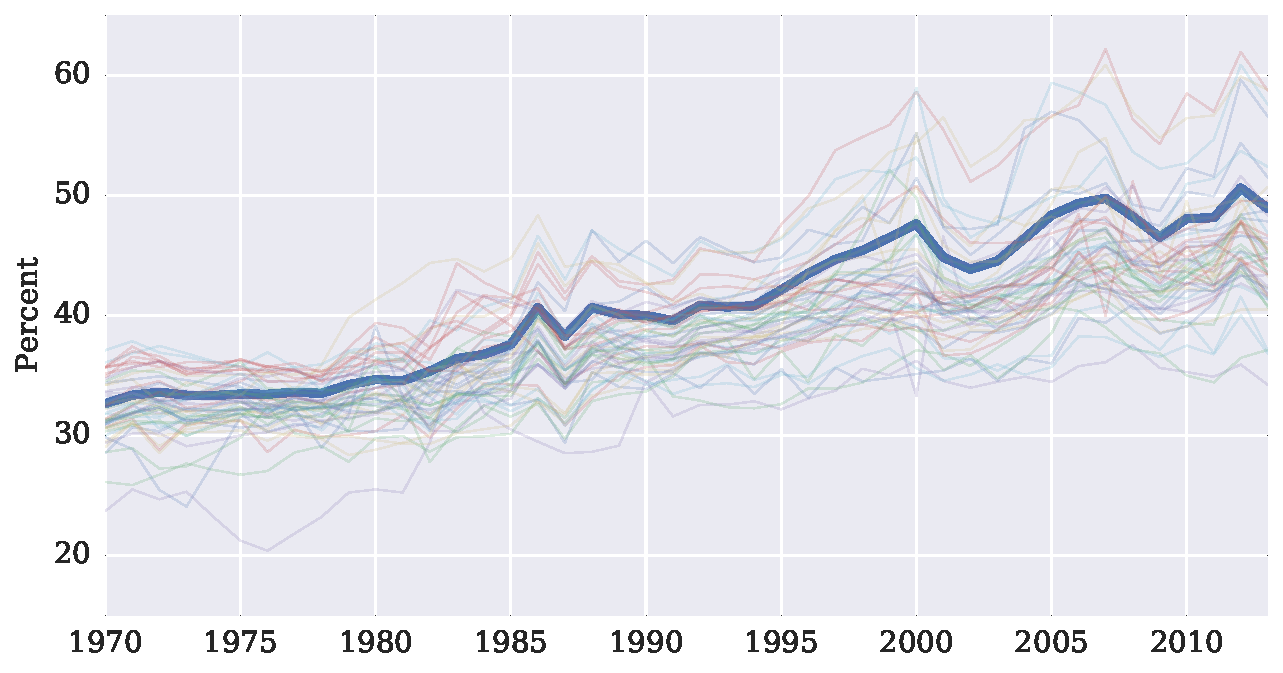
\includegraphics[width=4in]{../figures/inc_inequality/UnitedStates_Inc10_timeline.pdf}
  \end{center}
  \end{figure}


\end{frame}
%%%%%%%%%%%%%%%%%%%%%%%%%%%%%%%%%%%%%%%%%%%%%%%%%%%%%%%%%%%%%%%%%%%%%%%%%%%%%%%%%%%%%%%%%%%%%%%%%%%%%%%%%%%%%%%%%%%%%%%%%%%%%%%%%%%



%%%%%%%%%%%%%%%%%%%%%%%%%%%%%%%%%%%%%%%%%%%%%%%%%%%%%%%%%%%%%%%%%%%%%%%%%%%%%%%%%%%%%%%%%%%%%%%%%%%%%%%%%%%%%%%%%%%%%%%%%%%%%%%%%%%%
\begin{frame}
\frametitle{US Top 1\% Income Share (1970-2013) \widehrulefill}

  \begin{figure}[htb!]    
  \begin{center}  
  \hspace{-.4cm}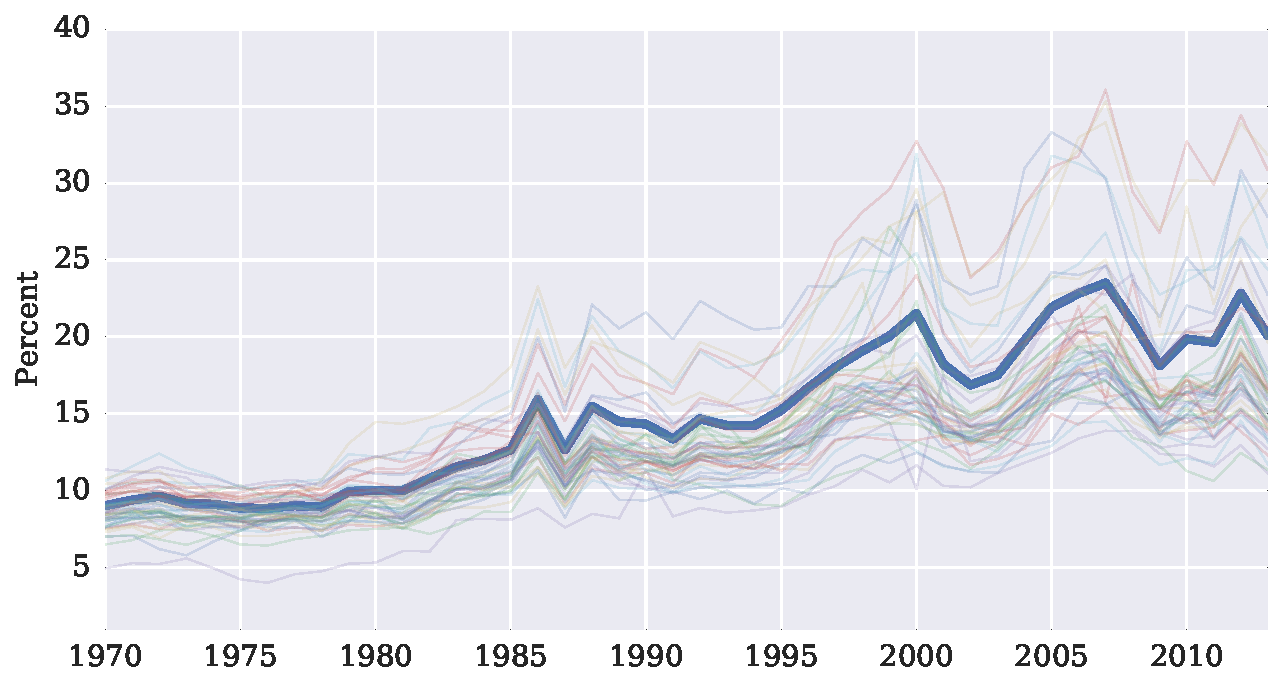
\includegraphics[width=4in]{../figures/inc_inequality/UnitedStates_Inc1_timeline.pdf}
  \end{center}
  \end{figure}


\end{frame}
%%%%%%%%%%%%%%%%%%%%%%%%%%%%%%%%%%%%%%%%%%%%%%%%%%%%%%%%%%%%%%%%%%%%%%%%%%%%%%%%%%%%%%%%%%%%%%%%%%%%%%%%%%%%%%%%%%%%%%%%%%%%%%%%%%%


%%%%%%%%%%%%%%%%%%%%%%%%%%%%%%%%%%%%%%%%%%%%%%%%%%%%%%%%%%%%%%%%%%%%%%%%%%%%%%%%%%%%%%%%%%%%%%%%%%%%%%%%%%%%%%%%%%%%%%%%%%%%%%%%%%%%
\begin{frame}
\frametitle{State Gini Coefficients (1970-2013)\widehrulefill}

  \begin{figure}[htb!]    
  \begin{center}  
  \hspace{-.4cm}\includegraphics[width=4in]{../figures/inc_inequality/UnitedStates_gini_timeline.pdf}
  \end{center}
  \end{figure}


\end{frame}
%%%%%%%%%%%%%%%%%%%%%%%%%%%%%%%%%%%%%%%%%%%%%%%%%%%%%%%%%%%%%%%%%%%%%%%%%%%%%%%%%%%%%%%%%%%%%%%%%%%%%%%%%%%%%%%%%%%%%%%%%%%%%%%%%%%


%%%%%%%%%%%%%%%%%%%%%%%%%%%%%%%%%%%%%%%%%%%%%%%%%%%%%%%%%%%%%%%%%%%%%%%%%%%%%%%%%%%%%%%%%%%%%%%%%%%%%%%%%%%%%%%%%%%%%%%%%%%%%%%%%%%%
\begin{frame}
\frametitle{Geographic clustering \widehrulefill}

  \begin{figure}[htb!]    
  \caption{Change in Top Decile Income Shares: 1970-1974 to 2009-2013 \label{fig:P10_map}}  
  \begin{center}  
  \includegraphics[width=4.2in]{../figures/maps/Inc10_map.pdf}
  \end{center}
  \end{figure}

\end{frame}
%%%%%%%%%%%%%%%%%%%%%%%%%%%%%%%%%%%%%%%%%%%%%%%%%%%%%%%%%%%%%%%%%%%%%%%%%%%%%%%%%%%%%%%%%%%%%%%%%%%%%%%%%%%%%%%%%%%%%%%%%%%%%%%%%%%


%%%%%%%%%%%%%%%%%%%%%%%%%%%%%%%%%%%%%%%%%%%%%%%%%%%%%%%%%%%%%%%%%%%%%%%%%%%%%%%%%%%%%%%%%%%%%%%%%%%%%%%%%%%%%%%%%%%%%%%%%%%%%%%%%%%%
\begin{frame}
\frametitle{Geographic clustering \widehrulefill}

  \begin{figure}[htb!]    
  \caption{Change in Gini Coefficients: 1970-1974 to 2009-2013 \label{fig:P10_map}}  
  \begin{center}  
  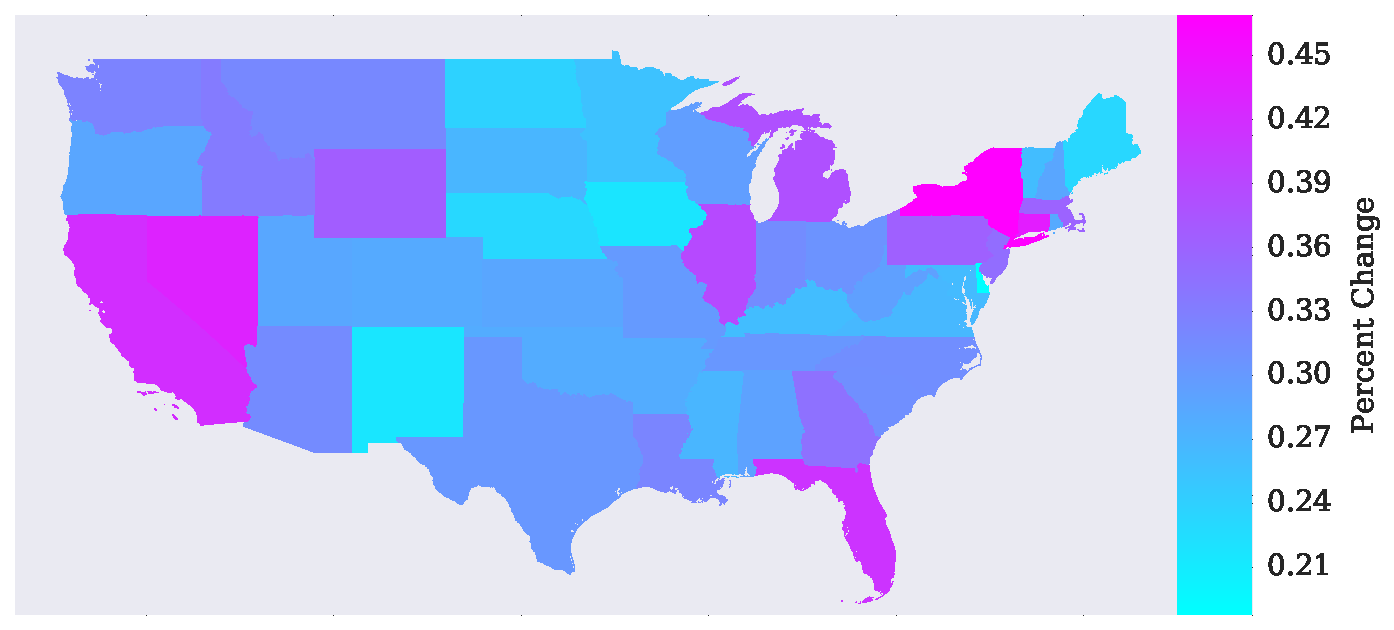
\includegraphics[width=4.2in]{../figures/maps/gini_map.pdf}
  \end{center}
  \end{figure}

\end{frame}
%%%%%%%%%%%%%%%%%%%%%%%%%%%%%%%%%%%%%%%%%%%%%%%%%%%%%%%%%%%%%%%%%%%%%%%%%%%%%%%%%%%%%%%%%%%%%%%%%%%%%%%%%%%%%%%%%%%%%%%%%%%%%%%%%%%




%%%%%%%%%%%%%%%%%%%%%%%%%%%%%%%%%%%%%%%%%%%%%%%%%%%%%%%%%%%%%%%%%%%%%%%%%%%%%%%%%%%%%%%%%%%%%%%%%%%%%%%%%%%%%%%%%%%%%%%%%%%%%%%%%%%%
\begin{frame}
\frametitle{Empirics \widehrulefill}
\begin{itemize}
\item Dependent variables:
  \begin{itemize}
    \smallskip
    \item Taxes: maximum income tax rates (NBER)
    \smallskip
    \item Entrepreneurship rates: age 0 firms per 100k people (Kauffman)
    \smallskip
    \item Demographics: percent black/retired, dependancy ratio (Census)
    \smallskip
    \item Technology: utility patent counts by state/year (USPTO)
    \smallskip
    \item Education: percent with high school/college (Frank 2009)
    \smallskip
    \item FIRE: share of employment (BEA)
  \end{itemize} 
\end{itemize}


\end{frame}
%%%%%%%%%%%%%%%%%%%%%%%%%%%%%%%%%%%%%%%%%%%%%%%%%%%%%%%%%%%%%%%%%%%%%%%%%%%%%%%%%%%%%%%%%%%%%%%%%%%%%%%%%%%%%%%%%%%%%%%%%%%%%%%%%%%


%%%%%%%%%%%%%%%%%%%%%%%%%%%%%%%%%%%%%%%%%%%%%%%%%%%%%%%%%%%%%%%%%%%%%%%%%%%%%%%%%%%%%%%%%%%%%%%%%%%%%%%%%%%%%%%%%%%%%%%%%%%%%%%%%%%%
\begin{frame}
\frametitle{Example: California Maximum Income Tax Rate \widehrulefill}

  \begin{figure}[htb!]    
  \begin{center}  
  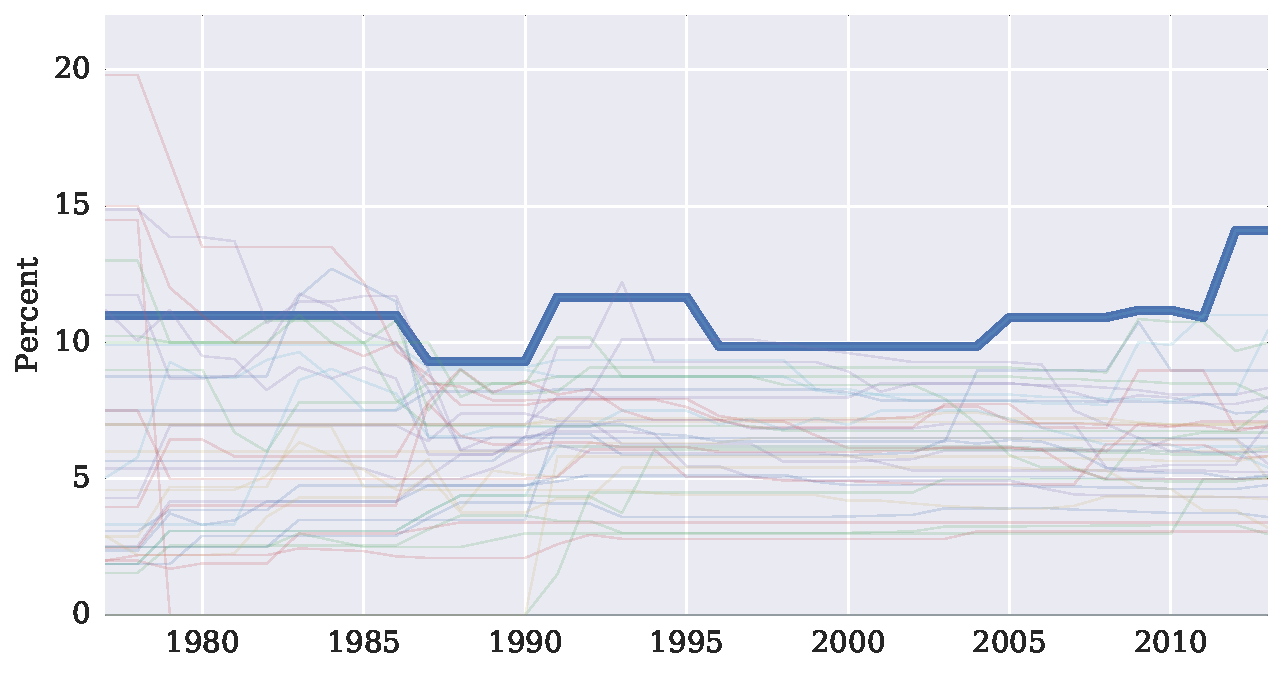
\includegraphics[width=4.2in]{../figures/tax_rates/California_MaxTaxRate_timeline.pdf}
  \end{center}
  \end{figure}

\end{frame}
%%%%%%%%%%%%%%%%%%%%%%%%%%%%%%%%%%%%%%%%%%%%%%%%%%%%%%%%%%%%%%%%%%%%%%%%%%%%%%%%%%%%%%%%%%%%%%%%%%%%%%%%%%%%%%%%%%%%%%%%%%%%%%%%%%%



%%%%%%%%%%%%%%%%%%%%%%%%%%%%%%%%%%%%%%%%%%%%%%%%%%%%%%%%%%%%%%%%%%%%%%%%%%%%%%%%%%%%%%%%%%%%%%%%%%%%%%%%%%%%%%%%%%%%%%%%%%%%%%%%%%%%
\begin{frame}
\frametitle{Example: California Entrepreneurship Rate \widehrulefill}

  \begin{figure}[htb!]    
  \caption{Age 0 firms per 100k people \label{fig:P10_map}}  
  \begin{center}  
  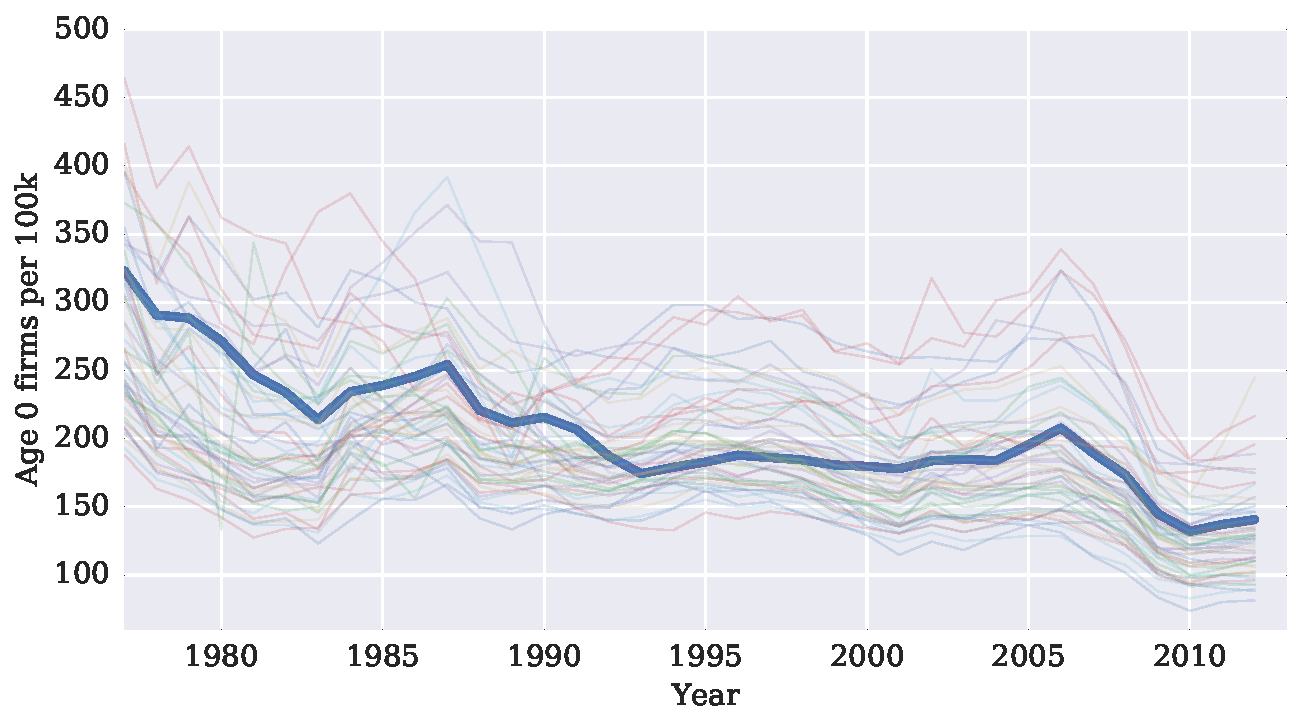
\includegraphics[width=4.2in]{../figures/entrep_data/California_startup_density.pdf}
  \end{center}
  \end{figure}

\end{frame}
%%%%%%%%%%%%%%%%%%%%%%%%%%%%%%%%%%%%%%%%%%%%%%%%%%%%%%%%%%%%%%%%%%%%%%%%%%%%%%%%%%%%%%%%%%%%%%%%%%%%%%%%%%%%%%%%%%%%%%%%%%%%%%%%%%%



%%%%%%%%%%%%%%%%%%%%%%%%%%%%%%%%%%%%%%%%%%%%%%%%%%%%%%%%%%%%%%%%%%%%%%%%%%%%%%%%%%%%%%%%%%%%%%%%%%%%%%%%%%%%%%%%%%%%%%%%%%%%%%%%%%%%
\begin{frame}
\frametitle{Example: California Patent Originiations \widehrulefill}

  \begin{figure}[htb!]    
  \caption{Utility Patents (i.e. patents for inventions) \label{fig:P10_map}}  
  \begin{center}  
  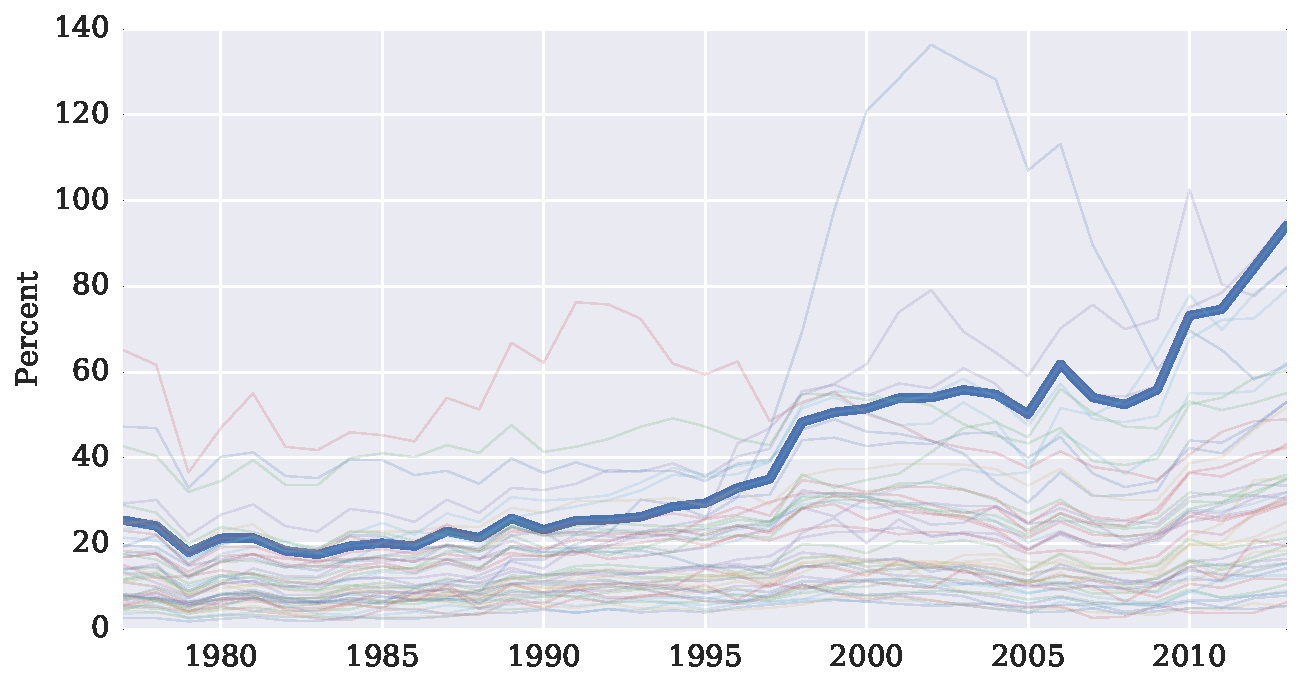
\includegraphics[width=4.2in]{../figures/patents/California_patents_timeline.pdf}
  \end{center}
  \end{figure}

\end{frame}
%%%%%%%%%%%%%%%%%%%%%%%%%%%%%%%%%%%%%%%%%%%%%%%%%%%%%%%%%%%%%%%%%%%%%%%%%%%%%%%%%%%%%%%%%%%%%%%%%%%%%%%%%%%%%%%%%%%%%%%%%%%%%%%%%%%





%%%%%%%%%%%%%%%%%%%%%%%%%%%%%%%%%%%%%%%%%%%%%%%%%%%%%%%%%%%%%%%%%%%%%%%%%%%%%%%%%%%%%%%%%%%%%%%%%%%%%%%%%%%%%%%%%%%%%%%%%%%%%%%%%%%%
\begin{frame}
\frametitle{Regression Exercises \widehrulefill}

\begin{itemize}
  \item Many variables/states are not stationary, so use approach from Pesaran et al (1997,1999)
  \msk
  \item Accounts for issues arising from cointegrated variables
\end{itemize}
%
\begin{eqnarray*}
\Delta y_{it} = \phi_{i}\left(y_{i,t-1} - \theta_i'X_{i,t} \right) +\sum_{j=1}^{n-1} \gamma^*_{ij} \Delta y_{i,t-j}+ \sum_{j=0}^{m-1} \beta^{*'}_{ij} \Delta X_{i,t-j} + \alpha_i +\varepsilon_{it}.
\end{eqnarray*}

\begin{itemize}
  \item Three estimators
  \begin{itemize}
    \item Fixed Effects (benchmark) - slope coefficients are fixed across states, intercepts vary
    \item Mean Group - average over individual state coefficients
    \item Pooled Group - long-run coefficients are fixed across states, short-run coefficients vary    
  \end{itemize}
\end{itemize}

\end{frame}
%%%%%%%%%%%%%%%%%%%%%%%%%%%%%%%%%%%%%%%%%%%%%%%%%%%%%%%%%%%%%%%%%%%%%%%%%%%%%%%%%%%%%%%%%%%%%%%%%%%%%%%%%%%%%%%%%%%%%%%%%%%%%%%%%%%




%%%%%%%%%%%%%%%%%%%%%%%%%%%%%%%%%%%%%%%%%%%%%%%%%%%%%%%%%%%%%%%%%%%%%%%%%%%%%%%%%%%%%%%%%%%%%%%%%%%%%%%%%%%%%%%%%%%%%%%%%%%%%%%%%%%%
\begin{frame}
\frametitle{Regression Results: Top 10\% Income Shares \widehrulefill}

\begin{small}
\begin{center}
\begin{tabular}{lccc} \hline 
 Variable & MG & PMG & FE \\ \hline 

WageTax\_total & -0.0132   & 0.0207   & -0.0141   \\
 & (0.0198)   & (0.0130)   & (0.0207)   \\
ent1 & 0.0764***   & -0.00611   & -0.0287   \\
 & (0.0215)   & (0.0163)   & (0.0336)   \\
pct\_black & 0.563***   & 0.0292**   & -0.0117   \\
 & (0.172)   & (0.0127)   & (0.0240)   \\
pct\_retired & 0.414***   & 0.196***   & 0.177**   \\
 & (0.111)   & (0.0307)   & (0.0808)   \\
patents\_percapita & 0.00119   & 0.0146*   & 0.0390***   \\
 & (0.0171)   & (0.00772)   & (0.0124)   \\
College & 0.159***   & 0.245***   & 0.237***   \\
 & (0.0473)   & (0.0195)   & (0.0389)   \\
fire\_pct & 0.112*   & 0.106***   & 0.101**   \\
 & (0.0627)   & (0.0286)   & (0.0431)   \\
&&&\\ \hline 

 Observations & 1,550 & 1,550 & 1,550 \\ 

 Num. groups  & 50 & 50 & 50 \\ 

\end{tabular} 
\end{center}
\end{small}
\end{frame}
%%%%%%%%%%%%%%%%%%%%%%%%%%%%%%%%%%%%%%%%%%%%%%%%%%%%%%%%%%%%%%%%%%%%%%%%%%%%%%%%%%%%%%%%%%%%%%%%%%%%%%%%%%%%%%%%%%%%%%%%%%%%%%%%%%%%




%%%%%%%%%%%%%%%%%%%%%%%%%%%%%%%%%%%%%%%%%%%%%%%%%%%%%%%%%%%%%%%%%%%%%%%%%%%%%%%%%%%%%%%%%%%%%%%%%%%%%%%%%%%%%%%%%%%%%%%%%%%%%%%%%%%%
\begin{frame}
\frametitle{Regression Results: Top 1\% Income Shares \widehrulefill}

\begin{small}
\begin{center}
\begin{tabular}{lccc} \hline 
 Variable & MG & PMG & DFE \\ \hline 

WageTax\_total & 0.0301*   & 0.0443***   & 0.0191   \\
 & (0.0175)   & (0.0130)   & (0.0225)   \\
ent1 & 0.167***   & 0.0763***   & 0.0410   \\
 & (0.0246)   & (0.0149)   & (0.0359)   \\
pct\_black & 0.284   & 0.0335***   & 0.0118   \\
 & (0.185)   & (0.0129)   & (0.0290)   \\
pct\_retired & 0.722***   & 0.413***   & 0.282***   \\
 & (0.132)   & (0.0368)   & (0.0915)   \\
patents\_percapita & 0.0331**   & 0.0162**   & 0.0283*   \\
 & (0.0156)   & (0.00721)   & (0.0159)   \\
College & 0.232***   & 0.290***   & 0.299***   \\
 & (0.0576)   & (0.0201)   & (0.0385)   \\
fire\_pct & -0.0121   & 0.0526*   & 0.0859**   \\
 & (0.0750)   & (0.0275)   & (0.0415)   \\
&&&\\ \hline 

 Observations & 1,550 & 1,550 & 1,550 \\ 

 Num. groups  & 50 & 50 & 50 \\ 

\end{tabular} 
\end{center}
\end{small}
\end{frame}
%%%%%%%%%%%%%%%%%%%%%%%%%%%%%%%%%%%%%%%%%%%%%%%%%%%%%%%%%%%%%%%%%%%%%%%%%%%%%%%%%%%%%%%%%%%%%%%%%%%%%%%%%%%%%%%%%%%%%%%%%%%%%%%%%%%%


%%%%%%%%%%%%%%%%%%%%%%%%%%%%%%%%%%%%%%%%%%%%%%%%%%%%%%%%%%%%%%%%%%%%%%%%%%%%%%%%%%%%%%%%%%%%%%%%%%%%%%%%%%%%%%%%%%%%%%%%%%%%%%%%%%%%
\begin{frame}
\frametitle{Regression Results: Gini Coefficients \widehrulefill}

\begin{small}
\begin{center}
\begin{tabular}{lccc} \hline 
 Variable & MG & PMG & DFE \\ \hline 

WageTax\_total & -0.274   & -0.277***   & -0.633***   \\
 & (0.222)   & (0.0450)   & (0.143)   \\
ent1 & 0.348   & 0.617***   & 0.648***   \\
 & (0.216)   & (0.0769)   & (0.154)   \\
pct\_black & 1.749   & 0.736***   & -0.0362   \\
 & (1.171)   & (0.120)   & (0.0529)   \\
pct\_retired & 0.497   & 0.0248   & 0.0751   \\
 & (0.995)   & (0.122)   & (0.160)   \\
patents\_percapita & 0.0108   & 0.0841***   & 0.0351   \\
 & (0.0857)   & (0.0202)   & (0.0440)   \\
College & 0.457   & 0.222***   & 0.263***   \\
 & (0.364)   & (0.0463)   & (0.0903)   \\
fire\_pct & 0.372   & 0.418***   & 0.349**   \\
 & (0.385)   & (0.0727)   & (0.154)   \\
&&&\\ \hline 

 Observations & 1,550 & 1,550 & 1,550 \\ 

 Num. groups  & 50 & 50 & 50 \\ 

\end{tabular} 
\end{center}
\end{small}
\end{frame}
%%%%%%%%%%%%%%%%%%%%%%%%%%%%%%%%%%%%%%%%%%%%%%%%%%%%%%%%%%%%%%%%%%%%%%%%%%%%%%%%%%%%%%%%%%%%%%%%%%%%%%%%%%%%%%%%%%%%%%%%%%%%%%%%%%%%




%%%%%%%%%%%%%%%%%%%%%%%%%%%%%%%%%%%%%%%%%%%%%%%%%%%%%%%%%%%%%%%%%%%%%%%%%%%%%%%%%%%%%%%%%%%%%%%%%%%%%%%%%%%%%%%%%%%%%%%%%%%%%%%%%%%%
\begin{frame}
\frametitle{Example: California Patent Originiations \widehrulefill}

  \begin{figure}[htb!]    
  \begin{center}  
  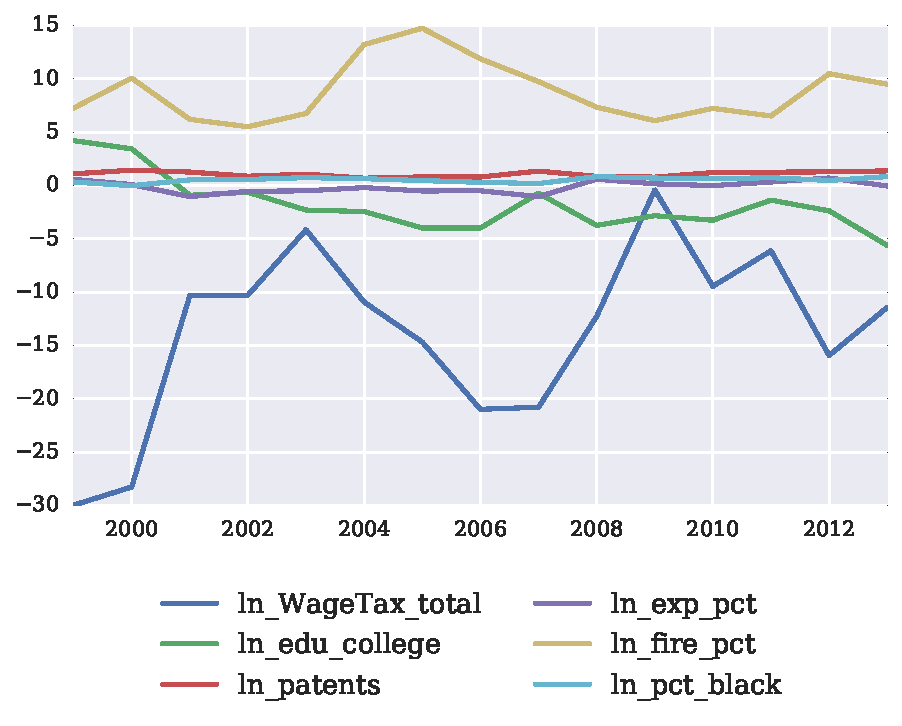
\includegraphics[width=4in]{../figures/top10_yearly_regs.pdf}
  \end{center}
  \end{figure}

\end{frame}
%%%%%%%%%%%%%%%%%%%%%%%%%%%%%%%%%%%%%%%%%%%%%%%%%%%%%%%%%%%%%%%%%%%%%%%%%%%%%%%%%%%%%%%%%%%%%%%%%%%%%%%%%%%%%%%%%%%%%%%%%%%%%%%%%%%



%%%%%%%%%%%%%%%%%%%%%%%%%%%%%%%%%%%%%%%%%%%%%%%%%%%%%%%%%%%%%%%%%%%%%%%%%%%%%%%%%%%%%%%%%%%%%%%%%%%%%%%%%%%%%%%%%%%%%%%%%%%%%%%%%%%%
\begin{frame}
\frametitle{Example: California Patent Originiations \widehrulefill}

  \begin{figure}[htb!]    
  \begin{center}  
  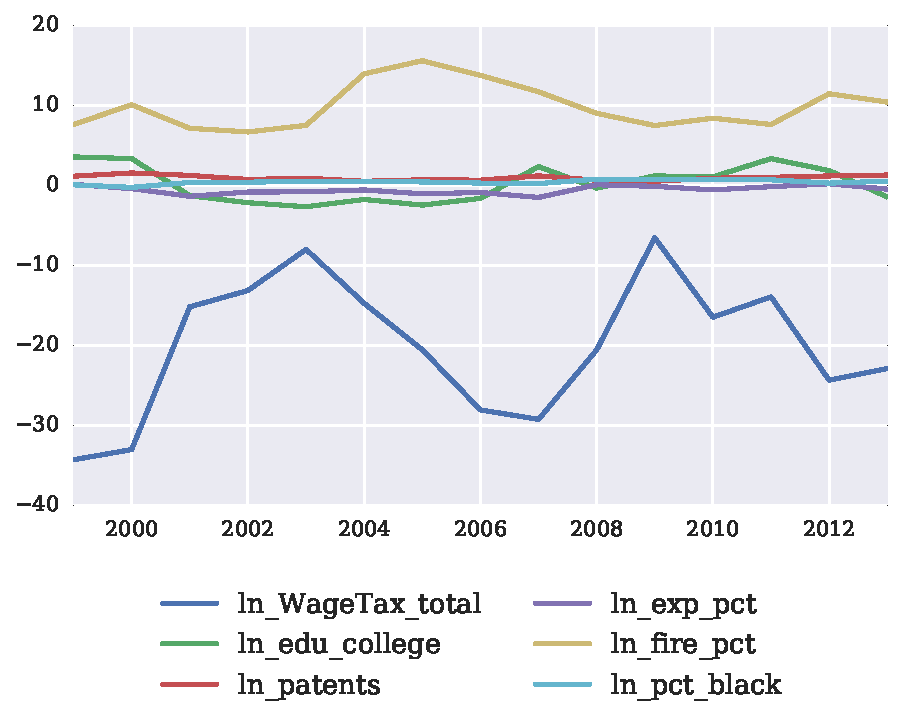
\includegraphics[width=4in]{../figures/top1_yearly_regs.pdf}
  \end{center}
  \end{figure}

\end{frame}
%%%%%%%%%%%%%%%%%%%%%%%%%%%%%%%%%%%%%%%%%%%%%%%%%%%%%%%%%%%%%%%%%%%%%%%%%%%%%%%%%%%%%%%%%%%%%%%%%%%%%%%%%%%%%%%%%%%%%%%%%%%%%%%%%%%




%%%%%%%%%%%%%%%%%%%%%%%%%%%%%%%%%%%%%%%%%%%%%%%%%%%%%%%%%%%%%%%%%%%%%%%%%%%%%%%%%%%%%%%%%%%%%%%%%%%%%%%%%%%%%%%%%%%%%%%%%%%%%%%%%%%%
\begin{frame}
\frametitle{Example: California Patent Originiations \widehrulefill}

  \begin{figure}[htb!]    
  \begin{center}  
  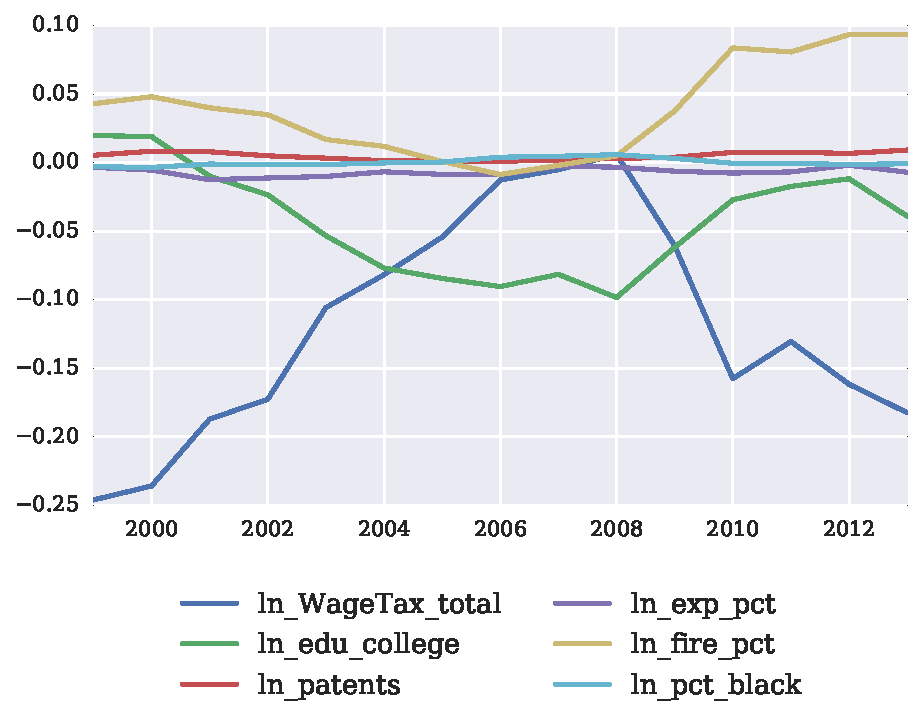
\includegraphics[width=4in]{../figures/gini_yearly_regs.pdf}
  \end{center}
  \end{figure}

\end{frame}
%%%%%%%%%%%%%%%%%%%%%%%%%%%%%%%%%%%%%%%%%%%%%%%%%%%%%%%%%%%%%%%%%%%%%%%%%%%%%%%%%%%%%%%%%%%%%%%%%%%%%%%%%%%%%%%%%%%%%%%%%%%%%%%%%%%







% %%%%%%%%%%%%%%%%%%%%%%%%%%%%%%%%%%%%%%%%%%%%%%%%%%%%%%%%%%%%%%%%%%%%%%%%%%%%%%%%%%%%%%%%%%%%%%%%%%%%%%%%%%%%%%%%%%%%%%%%%%%%%%%%%%%%
% \begin{frame}
% \frametitle{Model \widehrulefill}

% \begin{itemize}
%   \item Agents: 
%   \begin{itemize}
%     \item continuum of households
%     \msk
%     \item Finitely lived: $N$ overlapping generations
%   \end{itemize}

%   \bsk
%   \item Three major phases of life:
%   \begin{itemize}  
%     \msk
%     \item Endogenously invest in human capital 
%     \msk
%     \item Endogenously choose firm ownership, employ other households
%     \begin{itemize}
%       \item Hopenhayn \& Rogerson (1993)
%     \end{itemize}
%     \msk
%     \item Mandatory retirement and death, random bequests
%     \msk
%     \item Liquid savings earn fixed interest rate $r_t$
%   \end{itemize}

%   \bsk
%   \item Model object of interest, an income distribution
% \end{itemize}


% \end{frame}
% %%%%%%%%%%%%%%%%%%%%%%%%%%%%%%%%%%%%%%%%%%%%%%%%%%%%%%%%%%%%%%%%%%%%%%%%%%%%%%%%%%%%%%%%%%%%%%%%%%%%%%%%%%%%%%%%%%%%%%%%%%%%%%%%%%%




% %%%%%%%%%%%%%%%%%%%%%%%%%%%%%%%%%%%%%%%%%%%%%%%%%%%%%%%%%%%%%%%%%%%%%%%%%%%%%%%%%%%%%%%%%%%%%%%%%%%%%%%%%%%%%%%%%%%%%%%%%%%%%%%%%%%%
% \begin{frame}
% \frametitle{Phase 1 - Human Capital \widehrulefill}

% \begin{itemize}
%   \item Agents observe bequests $a_0\geq0$ and initial productivity signal $z_0$
%   \msk
%   \item Productivity is persistent AR(1), guides expectations
% \end{itemize}

% \begin{eqnarray*}
% &&\hat{V}_{h_0}(a_0,z_0,k_0)=\max_{hc} E_t\left[ \hat{V}^w_{h_1}(a_1,z_1,0)\right] \\
% \text{subject to}   && a_1 = a_0 - \psi(hc) \\
%           && z_1 = \rho_z z_0 + \sigma_z\epsilon_t + hc, \;\; \epsilon_t\sim N(0,1)
% \end{eqnarray*}


% \end{frame}
% %%%%%%%%%%%%%%%%%%%%%%%%%%%%%%%%%%%%%%%%%%%%%%%%%%%%%%%%%%%%%%%%%%%%%%%%%%%%%%%%%%%%%%%%%%%%%%%%%%%%%%%%%%%%%%%%%%%%%%%%%%%%%%%%%%%



% %%%%%%%%%%%%%%%%%%%%%%%%%%%%%%%%%%%%%%%%%%%%%%%%%%%%%%%%%%%%%%%%%%%%%%%%%%%%%%%%%%%%%%%%%%%%%%%%%%%%%%%%%%%%%%%%%%%%%%%%%%%%%%%%%%%%
% \begin{frame}
% \frametitle{Phase 2 - Working Life \widehrulefill}

% \begin{itemize}
%   \item Agents observe wealth $a_t$ and previous productivity signal $z_{t-1}$
%   \msk
%   \item Decide whether or not to enter period as a firm-owner or worker
%   \msk
%   \item Firm-owners and workers match to produce, invest in capital $i_t$
%   \msk
%   \item Workers receive a wage $w$, firm-owners earn profits $\pi$
%   \msk
%   \item All households make consumption/savings decisions

% \end{itemize}


% \end{frame}
% %%%%%%%%%%%%%%%%%%%%%%%%%%%%%%%%%%%%%%%%%%%%%%%%%%%%%%%%%%%%%%%%%%%%%%%%%%%%%%%%%%%%%%%%%%%%%%%%%%%%%%%%%%%%%%%%%%%%%%%%%%%%%%%%%%%



% %%%%%%%%%%%%%%%%%%%%%%%%%%%%%%%%%%%%%%%%%%%%%%%%%%%%%%%%%%%%%%%%%%%%%%%%%%%%%%%%%%%%%%%%%%%%%%%%%%%%%%%%%%%%%%%%%%%%%%%%%%%%%%%%%%%%
% \begin{frame}
% \frametitle{Phase 2.1 - Entry and Exit \widehrulefill}

% \begin{itemize}
%   \item Agents observe wealth $a_t$ and previous productivity signal $z_{t-1}$
%   \msk
%   \item Decide whether or not to enter period as a firm-owner or laborer
%   \msk
%   \item Entry cost $c_f$, initial capital $k_t = i_t$, capital adjustment costs $\Phi(0,k_t)$ 

%   \bsk
%   \item Incumbent firm-owner solves:
% \begin{small}
% \begin{eqnarray*}
% \hat{V}^f_{h_n}(a_t,z_{t-1},k_t)=\max\left\{ E_t\left[ V^w_{h_n}(a_t,z_t,0)-\Phi(0,k_t) \right],\; E_t\left[ V^f_{h_n}(a_t,z_t,k_t)\right]\right\}
% \end{eqnarray*}
% \end{small}

%   \item Incumbent worker solves:
% \begin{small}
% \begin{eqnarray*}
% \hat{V}^w_{h_n}(a_t,z_{t-1},0)=\max\left\{ E_t\left[ V^w_{h_n}(a_t,z_t,0) \right],\; E_t\left[ V^f_{h_n}(a_t,z_t,i_t)-c_f- i_t- \Phi(i_t,0)\right]\right\} 
% \end{eqnarray*}
% \end{small}

% \end{itemize}
% \end{frame}
% %%%%%%%%%%%%%%%%%%%%%%%%%%%%%%%%%%%%%%%%%%%%%%%%%%%%%%%%%%%%%%%%%%%%%%%%%%%%%%%%%%%%%%%%%%%%%%%%%%%%%%%%%%%%%%%%%%%%%%%%%%%%%%%%%%%



% %%%%%%%%%%%%%%%%%%%%%%%%%%%%%%%%%%%%%%%%%%%%%%%%%%%%%%%%%%%%%%%%%%%%%%%%%%%%%%%%%%%%%%%%%%%%%%%%%%%%%%%%%%%%%%%%%%%%%%%%%%%%%%%%%%%%
% \begin{frame}
% \frametitle{Phase 2.2 - Production \widehrulefill}

% \begin{itemize}
%   \item Agents observe wealth $a_t$, capital $k_t$ and productivity $z_{t}$
%   \msk
%   \item Workers evenly divide among firm-owners, earn wage $w(z_i,z_j)$
%   \msk
%   \item Firm owners choose investment, earn profits $\Pi$
%   \msk
%   \item Fixed cost for running business $c_j$
% \end{itemize}

% \begin{eqnarray*}
% y_i = z_j z_i^{1-\alpha} (k/n)^\alpha, \;\; \alpha\in(0,1).
% \end{eqnarray*}

% \begin{eqnarray*}
% \Pi_j(z_t, i_t, k_t,\{z_i\}) =  \int \left( y_i - w_i(z_i) \right) dZ - \Phi(i_t, k_t) - c_j.  
% \end{eqnarray*}


% \end{frame}
% %%%%%%%%%%%%%%%%%%%%%%%%%%%%%%%%%%%%%%%%%%%%%%%%%%%%%%%%%%%%%%%%%%%%%%%%%%%%%%%%%%%%%%%%%%%%%%%%%%%%%%%%%%%%%%%%%%%%%%%%%%%%%%%%%%%




% %%%%%%%%%%%%%%%%%%%%%%%%%%%%%%%%%%%%%%%%%%%%%%%%%%%%%%%%%%%%%%%%%%%%%%%%%%%%%%%%%%%%%%%%%%%%%%%%%%%%%%%%%%%%%%%%%%%%%%%%%%%%%%%%%%%%
% \begin{frame}
% \frametitle{Phase 2.3 - Consumption/Savings \widehrulefill}

% \begin{itemize}
%   \item After production, agents make consumption/savings decision
% \end{itemize}

% \begin{eqnarray*}
% && V^w_{h_n}(a_t,z_t,0) = \max_{c_t,a_{t+1}} u(c_t) + \beta E_t\left[ \hat{V}^w_{h_{n+1}}(a_{t+1},z_{t},0) \right] \\
% \text{subject to } && c_t + a_{t+1} \leq w_t + r_t a_t. 
% \end{eqnarray*}

% \begin{eqnarray*}
% && V^f_{h_n}(a_t,z_t,k_t) = \max_{c_t,a_{t+1},i_t} u(c_t) + \beta E_t\left[ \hat{V}^f_{h_{n+1}}(a_{t+1},z_{t},k_{t+1}) \right]  \\
% \text{subject to } && c_t + a_{t+1} \leq \Pi_t(i_t,k_t) + r_t a_t, \\
%            && k_{t+1} = k_t(1-\delta) + i_t 
% \end{eqnarray*}
% \end{frame}
% %%%%%%%%%%%%%%%%%%%%%%%%%%%%%%%%%%%%%%%%%%%%%%%%%%%%%%%%%%%%%%%%%%%%%%%%%%%%%%%%%%%%%%%%%%%%%%%%%%%%%%%%%%%%%%%%%%%%%%%%%%%%%%%%%%%



% %%%%%%%%%%%%%%%%%%%%%%%%%%%%%%%%%%%%%%%%%%%%%%%%%%%%%%%%%%%%%%%%%%%%%%%%%%%%%%%%%%%%%%%%%%%%%%%%%%%%%%%%%%%%%%%%%%%%%%%%%%%%%%%%%%%%
% \begin{frame}
% \frametitle{Phase 3 - Retirement and Death \widehrulefill}

% \begin{itemize}
%   \item Agents retire with certainty at age $h_R$, die at age $h_N$
%   \msk
%   \item Receives bequest motive with probability $\gamma$
%   \msk

%   \item If given a bequest motive
%   \begin{eqnarray*}
%   && V^b_{h_N}(a_t) = \max_{c_t,a_0} u(c_t) + \nu(a_0)\\
%   \text{subject to } && c_t + a_0 = a_t.
%   \end{eqnarray*}

%   \msk
%   \item If no bequest motive
%   \begin{eqnarray*}
%   && V_{h_N}(a_t) = \max_{c_t} u(c_t)\\
%   \text{subject to } && c_t = a_t
%   \end{eqnarray*}

% \end{itemize}
% \end{frame}
% %%%%%%%%%%%%%%%%%%%%%%%%%%%%%%%%%%%%%%%%%%%%%%%%%%%%%%%%%%%%%%%%%%%%%%%%%%%%%%%%%%%%%%%%%%%%%%%%%%%%%%%%%%%%%%%%%%%%%%%%%%%%%%%%%%%




% %%%%%%%%%%%%%%%%%%%%%%%%%%%%%%%%%%%%%%%%%%%%%%%%%%%%%%%%%%%%%%%%%%%%%%%%%%%%%%%%%%%%%%%%%%%%%%%%%%%%%%%%%%%%%%%%%%%%%%%%%%%%%%%%%%%%
% \begin{frame}
% \frametitle{Phase 3 - Retirement before Death \widehrulefill}

% \begin{itemize}
%   \item Second to last period
%   \begin{eqnarray*}
%   && V_{h_{N-1}}(a_t) = \max_{c_t, a_{t+1}} u(c_t) + \beta \left[ (1-\gamma)V_{h_N} + \gamma V^b_{h_N} \right]\\
%   \text{subject to } &&  c_t +a_{t+1} = r_ta_t
%   \end{eqnarray*}

%   \bsk
%   \item All previous periods in retirement
%   \begin{eqnarray*}
%   && V_{h_{n}}(a_t) = \max_{c_t, a_{t+1}} u(c_t) + \beta E_t\left[ V_{h_{n+1}}(a_t)\right], \\
%   \text{subject to } && c_t +a_{t+1} = r_ta_t.
%   \end{eqnarray*}



% \end{itemize}
% \end{frame}
% %%%%%%%%%%%%%%%%%%%%%%%%%%%%%%%%%%%%%%%%%%%%%%%%%%%%%%%%%%%%%%%%%%%%%%%%%%%%%%%%%%%%%%%%%%%%%%%%%%%%%%%%%%%%%%%%%%%%%%%%%%%%%%%%%%%




% %%%%%%%%%%%%%%%%%%%%%%%%%%%%%%%%%%%%%%%%%%%%%%%%%%%%%%%%%%%%%%%%%%%%%%%%%%%%%%%%%%%%%%%%%%%%%%%%%%%%%%%%%%%%%%%%%%%%%%%%%%%%%%%%%%%%
% \begin{frame}
% \frametitle{Model Results \widehrulefill}

% \begin{itemize}
%   \item Distribution of firm size (capital)
  
%   \msk
%   \item Distribution of income/savings  
%   \begin{itemize}
%     \item Can be examined across firms, age, initial human capital investment
%   \end{itemize}  
  
%   \msk
%   \item Model extensions:
%   \begin{itemize}
%      \item Taxes (easy)
%      \item Assortative matching between firms and households?
%    \end{itemize} 

%   \msk
%   \item Counterfactuals:
%   \begin{itemize}
%      \item Examine impact of demographic changes
%      \item Examine impact of changes in tax rates
%      \item Technological change (distribution of $z$?)
%    \end{itemize} 
% \end{itemize}


% \end{frame}
% %%%%%%%%%%%%%%%%%%%%%%%%%%%%%%%%%%%%%%%%%%%%%%%%%%%%%%%%%%%%%%%%%%%%%%%%%%%%%%%%%%%%%%%%%%%%%%%%%%%%%%%%%%%%%%%%%%%%%%%%%%%%%%%%%%%





% %%%%%%%%%%%%%%%%%%%%%%%%%%%%%%%%%%%%%%%%%%%%%%%%%%%%%%%%%%%%%%%%%%%%%%%%%%%%%%%%%%%%%%%%%%%%%%%%%%%%%%%%%%%%%%%%%%%%%%%%%%%%%%%%%%%%
% \begin{frame}
% \frametitle{Income Inequality \widehrulefill}

%   \begin{figure}[htb!]    
%   \begin{center}  
%   \caption{Nevada Top 10\% Income Share (1970-2013) \label{fig:P10_US_timeline}} 
  
%   \hspace{-.4cm}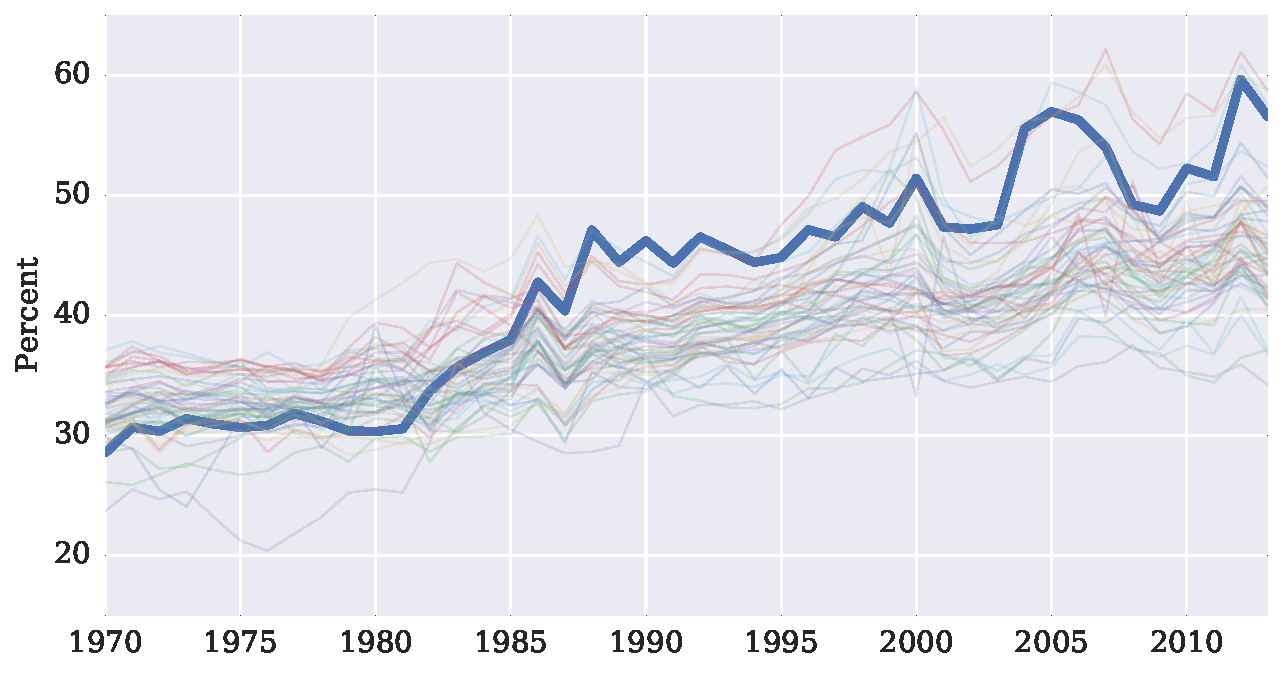
\includegraphics[width=4in]{../figures/inc_inequality/Nevada_Inc10_timeline.pdf}
%   \end{center}
%   \end{figure}


% \end{frame}
% %%%%%%%%%%%%%%%%%%%%%%%%%%%%%%%%%%%%%%%%%%%%%%%%%%%%%%%%%%%%%%%%%%%%%%%%%%%%%%%%%%%%%%%%%%%%%%%%%%%%%%%%%%%%%%%%%%%%%%%%%%%%%%%%%%%



% %%%%%%%%%%%%%%%%%%%%%%%%%%%%%%%%%%%%%%%%%%%%%%%%%%%%%%%%%%%%%%%%%%%%%%%%%%%%%%%%%%%%%%%%%%%%%%%%%%%%%%%%%%%%%%%%%%%%%%%%%%%%%%%%%%%%
% \begin{frame}
% \frametitle{Entrepreneurship \widehrulefill}

%   \begin{figure}[htb!]    
%   \begin{center}  
%   \caption{Pennsylvania Startup Density (1977-2013) \label{fig:P10_US_timeline}}  
%   \hspace{-.4cm}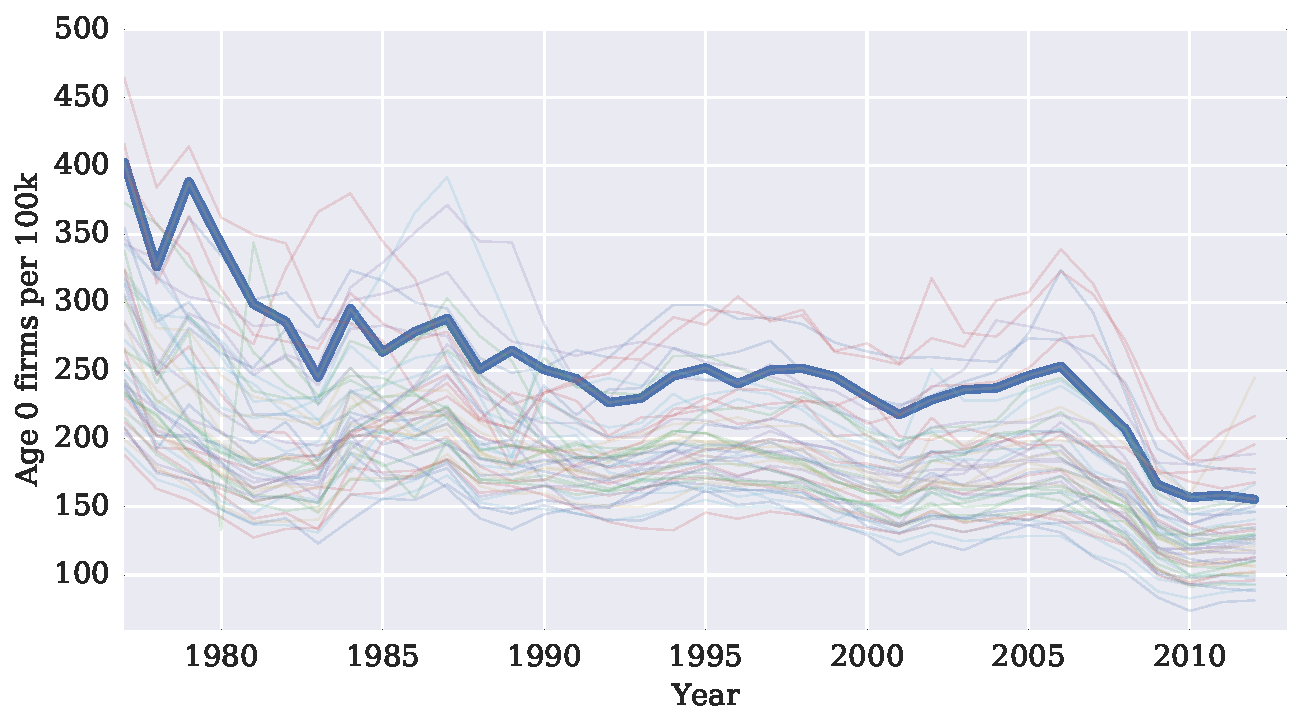
\includegraphics[width=4in]{../figures/entrep_data/Nevada_startup_density.pdf}
%   \end{center}
%   \end{figure}


% \end{frame}
% %%%%%%%%%%%%%%%%%%%%%%%%%%%%%%%%%%%%%%%%%%%%%%%%%%%%%%%%%%%%%%%%%%%%%%%%%%%%%%%%%%%%%%%%%%%%%%%%%%%%%%%%%%%%%%%%%%%%%%%%%%%%%%%%%%%



% %%%%%%%%%%%%%%%%%%%%%%%%%%%%%%%%%%%%%%%%%%%%%%%%%%%%%%%%%%%%%%%%%%%%%%%%%%%%%%%%%%%%%%%%%%%%%%%%%%%%%%%%%%%%%%%%%%%%%%%%%%%%%%%%%%%%
% \begin{frame}
% \frametitle{Entrepreneurship \widehrulefill}

%   \begin{figure}[htb!]    
%   \begin{center}  
%   \caption{Pennsylvania Startup Density (1977-2013) \label{fig:P10_US_timeline}}  
%   \hspace{-.4cm}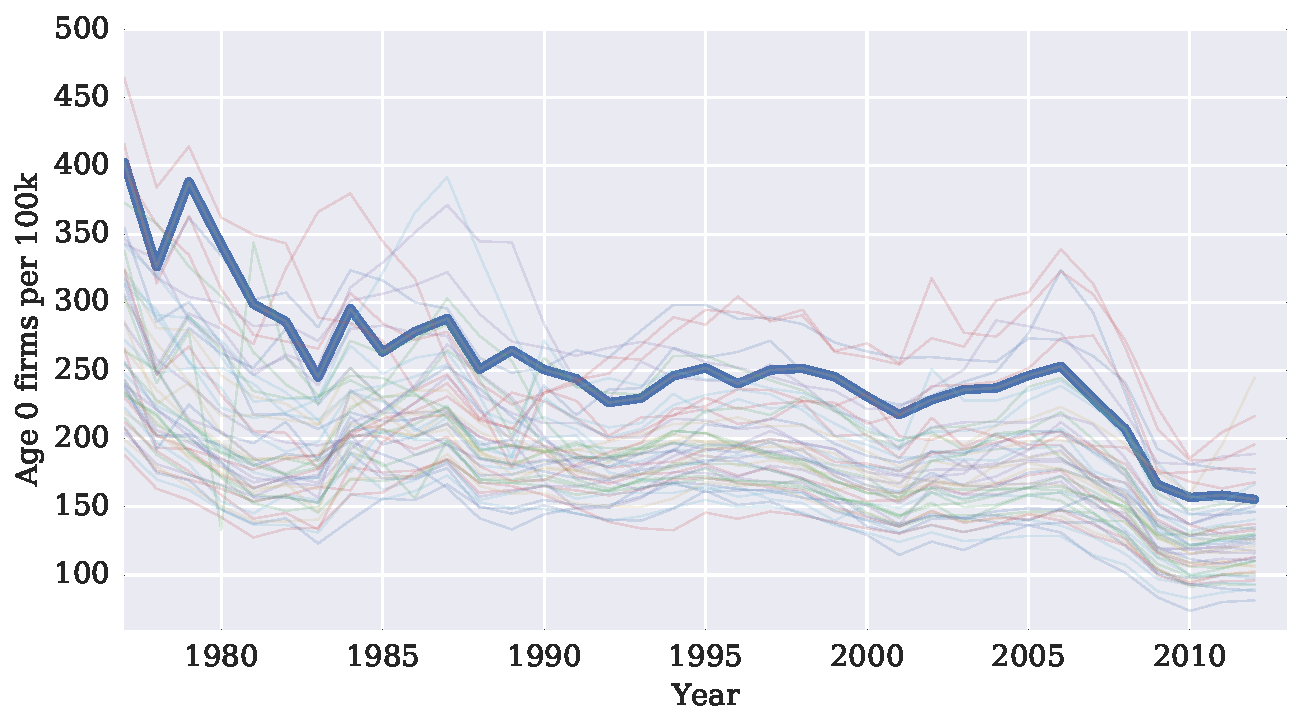
\includegraphics[width=4in]{../figures/entrep_data/Nevada_startup_density.pdf}
%   \end{center}
%   \end{figure}


% \end{frame}
% %%%%%%%%%%%%%%%%%%%%%%%%%%%%%%%%%%%%%%%%%%%%%%%%%%%%%%%%%%%%%%%%%%%%%%%%%%%%%%%%%%%%%%%%%%%%%%%%%%%%%%%%%%%%%%%%%%%%%%%%%%%%%%%%%%%



% %%%%%%%%%%%%%%%%%%%%%%%%%%%%%%%%%%%%%%%%%%%%%%%%%%%%%%%%%%%%%%%%%%%%%%%%%%%%%%%%%%%%%%%%%%%%%%%%%%%%%%%%%%%%%%%%%%%%%%%%%%%%%%%%%%%%
% \begin{frame}
% \frametitle{Geographic clustering \widehrulefill}

%   \begin{figure}[htb!]    
%   \caption{Change in Startup Density: 1977-1981 to 2009-2013 \label{fig:P10_map}}  
%   \begin{center}  
%   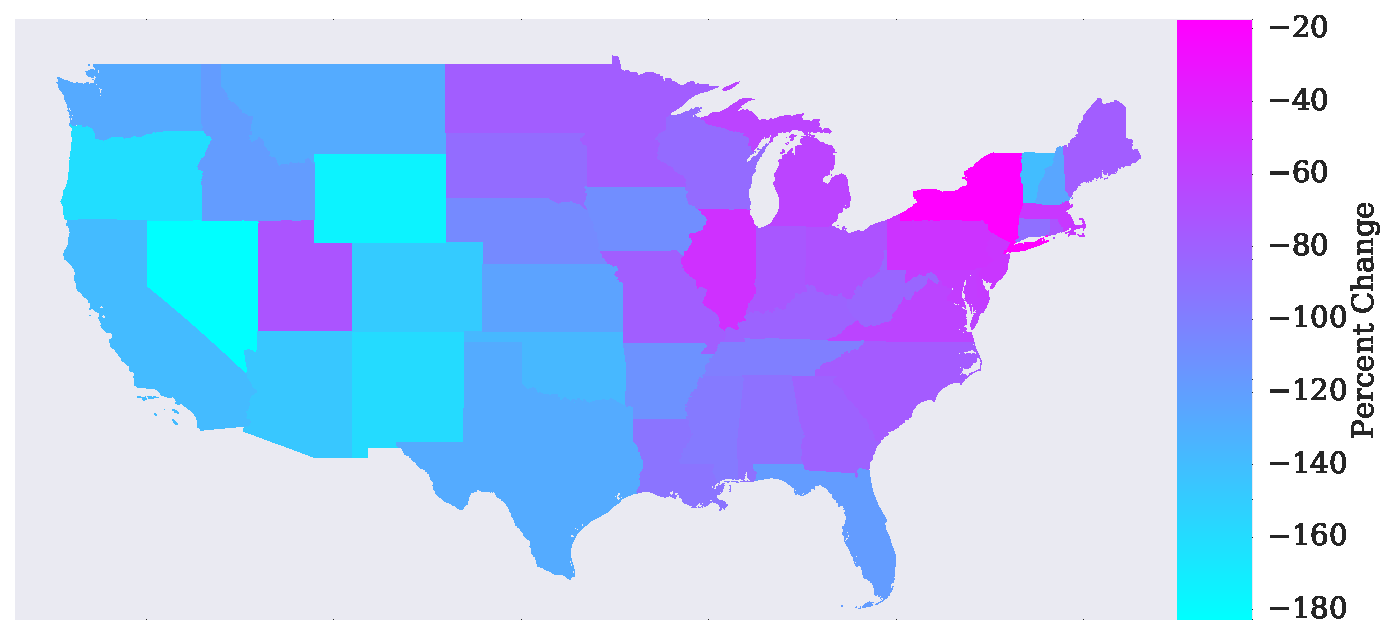
\includegraphics[width=4.2in]{../figures/maps/startupdensity_map.pdf}
%   \end{center}
%   \end{figure}

% \end{frame}
% %%%%%%%%%%%%%%%%%%%%%%%%%%%%%%%%%%%%%%%%%%%%%%%%%%%%%%%%%%%%%%%%%%%%%%%%%%%%%%%%%%%%%%%%%%%%%%%%%%%%%%%%%%%%%%%%%%%%%%%%%%%%%%%%%%%





\end{document}

